\documentclass[12pt]{beamer}
\usetheme{default} 

\setbeamertemplate{navigation symbols}{} %gets rid of navigation symbols
\setbeamertemplate{footline}{} %gets rid of bottom navigation bars
\setbeamertemplate{footline}[page number]{} %use this for page numbers

\setbeamertemplate{footline}{%
  \raisebox{5pt}{\makebox[\paperwidth]{\hfill\makebox[10pt]{\scriptsize\insertframenumber~~}}}}

\setbeamertemplate{itemize items}[circle] %round bullet points
\setlength\parskip{10pt} % white space between paragraphs

\usepackage{wrapfig}
\usepackage{subfig}
\usepackage{setspace}
\usepackage{enumerate}
\usepackage{graphicx}
\usepackage{amsmath}
\usepackage{amsfonts}
\usepackage{amssymb}
\usepackage{amsthm}
\usepackage[UKenglish]{isodate}
\usepackage{tikz}
\usepackage{pgfplots}
\usepackage{natbib}
\def\checkmark{\tikz\fill[scale=0.4](0,.35) -- (.25,0) -- (1,.7) -- (.25,.15) -- cycle;} 

% allow drawing arrows
\usetikzlibrary{arrows}
\tikzstyle{arrow}=[draw, -latex] 

% bracketing shortcuts
\newcommand{\paren}[1]{\left(#1\right)}
\newcommand{\sqbracket}[1]{\left[#1\right]}
\newcommand{\cbracket}[1]{\left\{#1\right\}}
\newcommand{\abs}[1]{\left\lvert#1\right\rvert}
\newcommand{\norm}[1]{\left\lVert#1\right\rVert}
% set up the argmin operator, argmax
\DeclareMathOperator*{\argmin}{arg\,min}
\DeclareMathOperator*{\argmax}{arg\,max}

\newcommand{\myframe}[1]{\begin{frame} \frametitle{#1}}
% the preamble
\title{Day 2, Session 1: Order of operations and negative numbers}
\author{Brian D. Williamson}
\institute{EPI/BIOST Bootcamp 2016}
\date{26 September 2016}

% Start the document
\begin{document}
% The title page
\begin{frame}
\titlepage
\end{frame}

\myframe{Outline for Session 1}
\begin{itemize}
\item Order of operations
\item[]
\item Negative numbers 
\item[]
\item Fractions
\item[]
\item Algebra
\item[]
\item Graphs
\end{itemize}
\end{frame}

\section{Order of operations}
\myframe{Evaluating expressions}
\begin{itemize}
\item Example expression: $3(1 + 2) + 5$
\item[]
\item How do we evaluate the above expression? In other words:
\begin{itemize}
\item Which terms to we compute first?
\item[]
\item Are there rules for evaluating expressions?
\end{itemize}
\end{itemize}
\end{frame}

\myframe{Order of operations}
\begin{itemize}
\item Rules for evaluating expressions:
\begin{enumerate}
\item Parentheses
\item Exponents
\item Multiplication and division
\item Addition and subtraction
\end{enumerate}
\item[]
\item A handy memory device: PEMDAS --- Please Excuse My Dear Aunt Sally
\end{itemize}
\end{frame}

\myframe{Example: order of operations in action!}
\begin{itemize}
\item Example from slide 2: $3(1 + 2) + 5$
\item[]
\item This notation is equivalent to $3\times (1+2) + 5$
\item[]
\item Apply PEMDAS: \hfill \underline{Current Expression}
\begin{enumerate}
\item Parentheses: add 1 and 2 \hfill $3(3) + 5$
\item Exponents: none \hfill $3(3) + 5$
\item Multiplication: multiply 3 and 3 \hfill $9 + 5$
\item Division: none \hfill $9 + 5$
\item Addition: add 9 and 5 \hfill 14
\item Subtraction: none
\end{enumerate}
\item[]
\item The final answer is 14!
\end{itemize}
\end{frame}

\myframe{Example: order of operations with exponents!}
\begin{itemize}
\item Expression: $\dfrac{(2^2 + 5)^2}{3\times 3} + 5$
\item[]
\item Apply PEMDAS: \hfill \underline{Current Expression}
\begin{enumerate}
\item Parentheses: $2^2 + 5$. \hfill $\frac{(2^2 + 5)^2}{3\times 3} + 5$
\item[] Need to apply PEMDAS again!
\begin{enumerate}
\item Parentheses: none \hfill $\frac{(2^2 + 5)^2}{3\times 3} + 5$
\item Exponents: $2^2 = 4$ \hfill $\frac{(4 + 5)^2}{3\times 3} + 5$
\item Multiplication/division: none \hfill $\frac{(4 + 5)^2}{3\times 3} + 5$
\item Addition/subtraction: $4 + 5 = 9$ \hfill $\frac{(9)^2}{3\times 3} + 5$
\end{enumerate}
\item Exponents: $9^2 = 81$ \hfill $\frac{81}{3\times 3} + 5$
\item Multiplication: $3 \times 3 = 9$ \hfill $\frac{81}{9} + 5$
\item Division: $81/9 = 9$ \hfill $9 + 5$
\item Addition/subtraction: $9 + 5 = 14$!
\end{enumerate}
\end{itemize}
\end{frame}

\myframe{Order of operations: nesting}
\begin{itemize}
\item Earlier, we needed to apply PEMDAS a second time, within the evaluation of the parentheses
\item[]
\item This is common!
\item[]
\item Apply PEMDAS as many times as necessary within each sub-expression, like $(2^2 + 5)$ in the previous example
\end{itemize}
\end{frame}

\myframe{Exercise: order of operations}
\begin{itemize}
\item Try to work out the following examples by yourself or in pairs:
\begin{enumerate}
\item $(5 \times 6) + 4$
\item[]
\item $5(4 - 2)^2$
\item[]
\item $[(2+1)^2 + 1]^2$
\end{enumerate}
\end{itemize}
\end{frame}

\myframe{Note on exercises}
\begin{itemize}
\item Solutions for the exercises are usually in the slides
\item[]
\item However, please attempt them first without looking at the solution!
\end{itemize}
\end{frame}

\myframe{Solution: order of operations}
\begin{enumerate}
\item $(5 \times 6) + 4 = 34$. PEMDAS:
\begin{itemize}
\item Parentheses: $5 \times 6$. Nested PEMDAS:
\begin{itemize}
\item Multiplication: $5 \times 6 = 30$
\end{itemize}
\item Addition: $30 + 4 = 34$
\end{itemize}
\item[]
\item $5(4 - 2)^2 = 20$. PEMDAS:
\begin{itemize}
\item Parentheses: $4 - 2$. Nested PEMDAS:
\begin{itemize}
\item Subtraction: $4 - 2 = 2$
\end{itemize}
\item Exponents: $2^2 = 4$
\item Multiplication: $5 \times 4 = 20$
\end{itemize}
\item[]
\item $[(2+1)^2 + 1]^2 = 100$. PEMDAS:
\begin{itemize}
\item Parentheses: $(2 + 1)^2 + 1$. Nested PEMDAS:
\begin{itemize}
\item Parentheses: $2 + 1$. Nested PEMDAS --- Addition: $2 + 1 = 3$
\item Exponent: $3^2 = 9$ 
\item Addition: $9 + 1 = 10$
\end{itemize}
\item Exponent: $10^2 = 100$
\end{itemize}
\end{enumerate}
\end{frame}

\section{Negative numbers}
\myframe{Negative numbers: what are they?}
\begin{itemize}
\item Ways to think about negative numbers:
\begin{itemize}
\item A positive number subtracted from zero
\item[]
\item Opposites of positive numbers: $-4 + 4 = 0$
\item[]
\item Movement left on the number line
\end{itemize}
\end{itemize}
\end{frame}

\myframe{The number line}
\begin{itemize}
\item Movement on the number line:
\begin{itemize}
\item Right (positive numbers): 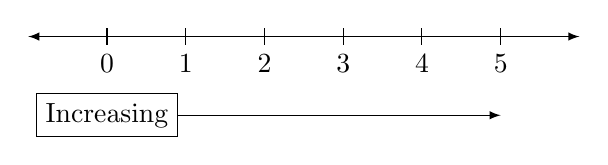
\begin{tikzpicture}
\draw[latex-latex] (-1, 0) -- (6, 0) ; %edit here for the axis
\foreach \x in  {0,1,2,3,4,5} % edit here for the vertical lines
\draw[shift={(\x,0)},color=black] (0pt,3pt) -- (0pt,-3pt);
\foreach \x in {0,1,2,3,4,5} % edit here for the numbers
\draw[shift={(\x,0)},color=black] (0pt,0pt) -- (0pt,-3pt) node[below] 
{$\x$};
\node[draw] (inc) at (0, -1) {Increasing};
\path [arrow] (inc) -- (5, -1);
\end{tikzpicture}
\item[]
\item Left (negative numbers): 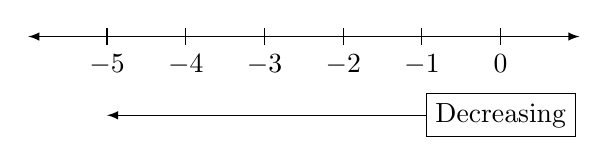
\begin{tikzpicture}
\draw[latex-latex] (-6, 0) -- (1, 0) ; %edit here for the axis
\foreach \x in  {0,-1,-2,-3,-4,-5} % edit here for the vertical lines
\draw[shift={(\x,0)},color=black] (0pt,3pt) -- (0pt,-3pt);
\foreach \x in {0,-1,-2,-3,-4,-5} % edit here for the numbers
\draw[shift={(\x,0)},color=black] (0pt,0pt) -- (0pt,-3pt) node[below] 
{$\x$};
\node[draw] (dec) at (0, -1) {Decreasing};
\path [arrow] (dec) -- (-5, -1);
\end{tikzpicture}
\end{itemize}
\item[]
\item Example: move left 3, starting at 100?
\begin{itemize}
\item Subtract 3
\item Add negative 3
\end{itemize}
\end{itemize}
\end{frame}

\myframe{Properties of negative numbers}
\begin{itemize}
\item Represent opposites of positive numbers, or movement left on the number line
\item[]
\item Subtraction = adding a negative number
\item[]
\item The product of two negatives is a positive
\item[]
\item Movement left on the numberline $\rightarrow$ smaller numbers
\end{itemize}
\end{frame}

\myframe{Example: two negatives make a positive}
\begin{itemize}
\item Expression: $-1 \times -1$
\item[]
\item Answer: 1!
\item[]
\item Why?
\begin{itemize}
\item $-1$ is a negative number
\item[]
\item Negative numbers mean opposites; the opposite of $-1$ is 1
\end{itemize}
\end{itemize}
\end{frame}

\myframe{Example: ordering negative numbers}
\begin{itemize}
\item Expression: $-3 \ \rule{.5cm}{0.15mm} \ -2$
\item[]
\item Answer: $-3 < -2$
\item[]
\item Why?
\begin{itemize}
\item Negative numbers are left motion on number line! -3 is further left than -2
\end{itemize}
\end{itemize}
\end{frame}

\myframe{Exercise: negative numbers}
\begin{itemize}
\item Try to work out the following examples by yourself or in pairs:
\begin{enumerate}
\item $-5.2 - (-11.3)$
\item[]
\item $-5 - 6$
\item[]
\item $(-1)\times(-5) + (-3)$
\end{enumerate}
\end{itemize}
\end{frame}

\myframe{Solution: negative numbers}
\begin{enumerate}
\item $-5.2 - (-11.3) = 6.1$
\begin{itemize}
\item $-(-11.3) = -1 \times (-11.3) = 11.3$
\item $-5.2 + 11.3 = 11.3 - 5.2 = 6.1$
\end{itemize}
\item[]
\item $-5 - 6 = -11$
\item[]
\item $(-1)\times(-5) + (-3) = 2$
\begin{itemize}
\item $-1 \times (-5) = 5$
\item $5 + (-3) = 5 - 3 = 2$
\end{itemize}
\end{enumerate}
\end{frame}

\myframe{Related concepts: absolute value}
\begin{itemize}
\item Magnitudes: how ``large'' is a number, with no direction
\begin{itemize}
\item Examples: speed (how fast an object is moving), length 
\end{itemize}
\item[]
\item Symbol for absolute value is $|\cdot |$
\end{itemize}
\centering
\begin{tikzpicture}
        \begin{axis}[%
            domain = -1:1,
            range = -1:1,
            samples = 50,
            axis x line = center,
            axis y line = center,
            xlabel = {$x$},
            ylabel = {$y$},
            ticks = none
            ]
            \addplot[blue] {abs(x)} [yshift=3pt] node[pos=.95,left] {$y=|x|$};
        \end{axis}
    \end{tikzpicture}
\end{frame}

\myframe{Example: absolute value of a positive number}
\begin{itemize}
\item Expression: $|4|$
\item[]
\item Answer is 4! Positive numbers already measure size, with no direction
\end{itemize}
\end{frame}

\myframe{Example: absolute value of a negative number}
\begin{itemize}
\item Expression: $|-4|$
\item[]
\item Answer is 4!
\item[]
\item Why?
\begin{itemize}
\item Negatives are opposites of positives
\item Absolute value has no direction
\item 4 and $-4$ are equally far away from zero
\end{itemize}
\end{itemize}
\end{frame}

\myframe{Related concepts: negative numbers and inequalities}
\begin{itemize}
\item Expression from before: $-3 < -2$
\item[]
\item What happens if we multiply both sides by $-1$?
\item[]
\item Negatives are opposites: signs change and inequality flips, yielding $2 < 3$
\end{itemize}
\end{frame}

\myframe{Exercise: absolute value, negative numbers}
\begin{itemize}
\item Try to work out the following examples by yourself or in pairs:
\begin{enumerate}
\item $|-5|$ and $|5|$
\item[]
\item Is $|-5| < 4$?
\item[]
\item Is $-15 > -14$? 
\item[]
\item Is $-(3 + 1)\times 5 < -(4 + 1)\times 3$?
\end{enumerate}
\end{itemize}
\end{frame}

\myframe{Solution: absolute value, negative numbers}
\begin{enumerate}
\item $|-5| = |5| = 5$
\item[]
\item $|-5| = 5$, and $5 > 4$; answer is no
\item[]
\item $-15$ is further from 0 than $-14$; also, 14 < 15. Hence $-15 < -14$
\item[]
\item Two ways to solve this:
\begin{itemize}
\item $-(3+1)\times 5 = -1\times(4)\times 5 = -20$, and $-(4+1)\times 3 = -1\times (5) \times 3 = -15$. So $-20 < -15$
\item[]
\item If $-(3+1)\times 5 < -(4+1)\times 3$, then $(3+1)\times 5 > (4+1)\times 3$. But this means $20 > 15$, which is true!
\end{itemize}
\end{enumerate}
\end{frame}
\end{document}
